\section{Expression Obsession}{\label{sec:expressionobsession}}
\begin{topics}
\verb!repeat! statement, variables and their data types (\verb!int, double!), mathematical functions \\(\verb!min, max, sqrt, pow, log, sine...!).
\end{topics}
\subsection{Harmonic Number}{\label{pp:harmonic}}
The $n$-th Harmonic Number ($H_n$) is the sum of the reciprocals of the first n natural numbers.
\begin{equation}
{H_{n}=1+{\frac {1}{2}}+{\frac {1}{3}}+\cdots +{\frac {1}{n}}=\sum _{i=1}^{n}{\frac {1}{i}}}
\end{equation}
\begin{fact}
The Harmonic series diverges; i.e., $H_n \rightarrow\infty$ as $n\rightarrow\infty$.
\end{fact}
\textbf{Problem Statement:}\\
Calculate $H_n$ for all test cases accurate till 10 decimal places. See Starter code (below) for more details.
\begin{testcases}
	{$t$ \hfill(number of test cases, an integer)\\
	$n_1\ n_2\ \ldots\ n_t$ \hfill($t$ space seperated integers for each testcase)}
	{$H_{n_i}$ \hfill(each test case on a newline, accurate till 10 decimal places)}
	{$1 \leq n_i \leq 10^{6}$}
	{11\\1 2 3 5 10 20 30 50 100 1000 1000000}
	{1.0000000000\\1.5000000000\\1.8333333333\\2.2833333333\\2.9289682540\\3.5977396571\\3.9949871309\\4.4992053383\\5.1873775176\\7.4854708606\\14.3927267229}
	{https://github.com/paramrathour/CS-101/tree/main/Starter Codes/Harmonic Number.cpp}
\end{testcases}
\begin{funvideo}
\href{https://youtu.be/Dgcoa2yAUfw}{The Harmonic Series -- Tipping Point Math}
\end{funvideo}
% \\\href{https://youtu.be/4k1jegU4Wb4}{The mystery of 0.577 -- Numberphile}
\subsection{Wallis Product}{\label{pp:wallis}}
$\pi/2$ is given by below infinite product formula. It is the ratio of product of even squares and odd squares
\begin{equation}
\frac{\pi}{2} = {\frac {2}{1}}\cdot {\frac {2}{3}}\cdot {\frac {4}{3}}\cdot {\frac {4}{5}}\cdot {\frac {6}{5}}\cdot {\frac {6}{7}}\cdots= \prod _{i=1}^{\infty}\left({\frac {2i}{2i-1}}\cdot {\frac {2i}{2i+1}}\right)
\end{equation}
Let's define $\pi_n$ as $n$-th iteration of this infinite product as below
\begin{equation*}
\frac{\pi_n}{2} = {\frac {2}{1}}\cdot {\frac {2}{3}}\cdot {\frac {4}{3}}\cdot {\frac {4}{5}}\cdot {\frac {6}{5}}\cdot {\frac {6}{7}}\cdots{\frac {2n}{2n-1}}\cdot {\frac {2n}{2n+1}} = \prod _{i=1}^{n}\left({\frac {2i}{2i-1}}\cdot {\frac {2i}{2i+1}}\right)
\end{equation*}
\textbf{Problem Statement:}\\
Calculate $\pi_n$ for all test cases accurate till 10 decimal places. See Starter code (below) for more details.
\begin{testcases}
	{$t$ \hfill(number of test cases, an integer)\\$n_1\ n_2\ \ldots\ n_t$ \hfill($t$ space seperated integers for each testcase)}
	{$\pi_{n_i}$ \hfill(each test case on a newline, accurate till 10 decimal places)}
	{$1 \leq n_i \leq 10^{6}$}
	{11\\1 2 3 5 10 20 30 50 100 1000 1000000}
	{2.6666666667\\2.8444444444\\2.9257142857\\3.0021759546\\3.0677038066\\3.1035169615\\3.1159482859\\3.1260789002\\3.1337874906\\3.1408077460\\3.1415918682}
	{https://github.com/paramrathour/CS-101/tree/main/Starter Codes/Wallis Product.cpp}
\end{testcases}
\begin{funvideo}
\href{https://youtu.be/8GPy_UMV-08}{The Wallis product for pi, proved geometrically -- 3Blue1Brown}
\end{funvideo}
\subsection{Tetration}{\label{pp:tetration}}
Problem \ref{pp:harmonic} is about repeated additions whereas \ref{pp:wallis} is about repeated multiplication. Guess what's this problem about. Yes! It's repeated exponentiation. Tetration, the next \href{https://en.wikipedia.org/wiki/Hyperoperation}{hyperoperation} after exponentiation defined as:%. It is defined as repeated exponentiation
\begin{equation}
{^{n}a}=\underbrace {a^{a^{\cdot ^{\cdot ^{a}}}}} _{n} \quad\text{repeated exponentiation}
\end{equation}
\textbf{Problem Statement:}\\
Calculate ${^{n}a}$ for all test cases accurate till 10 decimal places. See Starter code (below) for more details.
\begin{testcases}
	{$t$ \hfill(number of test cases, an integer)\\
	$a_1\ n_1\quad a_2\ n_2\quad \ldots\quad a_t\ n_t$ \hfill($t$ space seperated pairs for each testcase)}
	{${^{n}a}$ \hfill(each test case on a newline, accurate till 10 decimal places)}
	{$0.05 \leq a_i \leq 3$\hfill(a double)\\
	$1 \leq n_i \leq 1000$ \hfill(an integer)}
	{10\\1 1\quad1 2\quad2 1\quad2 2\quad2 3\quad3 2\quad3 3\quad1.41421356237 20\quad0.06598803584 1000 \quad	1.44466786101 1000}
	{1.0000000000\\1.0000000000\\2.0000000000\\4.0000000000\\16.0000000000\\27.0000000000\\7625597484987.0000000000\\1.9995856229\\0.3968311347\\2.7128728643}
	{https://github.com/paramrathour/CS-101/tree/main/Starter Codes/Tetration.cpp}
\end{testcases}
\begin{funvideo}
\href{https://youtu.be/0poh3w_Vm_A}{Tetration: The operation you were (probably) never taught -- Taylor Series}
\\\href{https://youtu.be/DmP3sFIZ0XE}{``Prove'' 4 = 2 Using Infinite Exponents. Can You Spot The Mistake? -- Mind Your Decisions}
\end{funvideo}
\subsection{Ramanujan's Nested Radical}{\label{pp:ramanujanradical}}
\begin{equation}
{ r={\sqrt{1+2{\sqrt{1+3{\sqrt{1+4{\sqrt{1+\cdots }} }}}}}} = \lim_{n\rightarrow\infty} {\sqrt {1+2{\sqrt {1+3{\sqrt {\cdots \sqrt{1+ n}}}}}}}}
\end{equation}
Let's define $r_n$ as $n$-th iteration of this infinite nested radical as below
\begin{equation*}
{ r_n={\sqrt {1+2{\sqrt {1+3{\sqrt {\cdots \sqrt{1+ n}}}}}}}}
\end{equation*}
\textbf{Problem Statement:}\\
Calculate $r_n$ for all test cases accurate till 10 decimal places. See Starter code (below) for more details.
\begin{testcases}
	{$t$ \hfill(number of test cases, an integer)\\$n_1\ n_2\ \ldots\ n_t$ \hfill($t$ space seperated integers for each testcase)}
	{$r_{n_i}$ \hfill(each test case on a newline, accurate till 10 decimal places)}
	{$2 \leq n_i \leq 100$}
	{8\\2 3 5 10 20 30 50 100}
	{1.7320508076\\2.2360679775\\2.7550532613\\2.9899203606\\2.9999878806\\2.9999999868\\3.0000000000\\3.0000000000}
	{https://github.com/paramrathour/CS-101/tree/main/Starter Codes/Ramanujan's Nested Radical.cpp}
\end{testcases}
\begin{funvideo}
\href{https://youtu.be/leFep9yt3JY}{Ramanujan's infinite root and its crazy cousins -- Mathologer}
\end{funvideo}
\subsection{Simple Continued Fractions}{\label{pp:simplecontinuedfractions}}
{A (finite) simple continued fraction of a rational number $r$ is defined using $n+1$ coefficients = $[a_0; a_1, a_2,\ldots, a_{n-1}, a_n]$.
% \begin{equation}
% { r=a_{0}+{\cfrac {1}{a_{1}+{\cfrac {1}{a_{2}+{\cfrac {1}{a_{3}+{_{\ddots }}}}}}}}}
% \end{equation}
% Let's define $r_n$ as $n$-th iteration of this infinite continued fraction as below
\\They can be expressed in \href{https://en.wikipedia.org/wiki/Generalized_continued_fraction#Notation}{Gauss' Kettenbruch notation} as follows
\begin{equation}
{ r=a_{0}+{\underset {i=1}{\overset {n }{\mathrm {K} }}}{\frac {1}{a_{n}}}\triangleq a_{0}+{\cfrac {1}{a_{1}+{\cfrac {1}{a_{2}+{\cfrac {1}{\ddots{+{\cfrac{1}{a_n} }}}}}}}} }
\end{equation}
\textbf{Problem Statement:}\\
Express $r$ as a quotient $p/q$ where $p,q$ are integers and $q\neq0$. See Starter code (below) for more details.
\begin{testcases}
	{$t$ \hfill(number of test cases, an integer)\\%This is followed by $t$ test cases (each testcase takes two lines)\\
	$n_i\quad a_{n_i}\ a_{n_{i-1}}\ \ldots\ a_1\ a_0$ \hfill($n_i+2$ space seperated integers for each testcase)}
	{$p_{n_i}/q_{n_i}$ \hfill(each test case on a newline, where $r_{n_i} = p_{n_i}/q_{n_i}$ (in irreducible form))
	% If $q_{n_i}=1$, output only $p_{n_i}$
	}
	{$0 \leq n_i \leq 50$\\
	$a_{0}$ is an integer whereas $a_1, a_2, \ldots, a_{n_i -1}, a_{n_i}$ are positive integers\\
	$a_0, a_1, a_2, \ldots, a_{n_i -1}, a_{n_i}$ are such that $-2,147,483,648\leq p_{n_i},q_{n_i}\leq2,147,483,647$\hfill(C++'s \texttt{int} range)% \hfill(i.e., $p_{n_i},q_{n_i}$ are within the range of C++'s int data type)
	}
	% $\leq a_{n_i} \leq$}
	{11\\0 0\\1 1 0\\1 1 1\\1 7 3\\8 1 1 1 1 1 1 1 1 1\\10 1 1 1 1 1 1 1 1 1 2 -2\\3 1 15 7 3\\9 13 3 4 1 2 1 2 1 1 0\\12 14 1 3 1 2 1 1 1 292 1 15 7 3\\22 1 1 14 1 1 12 1 1 10 1 1 8 1 1 6 1 1 4 1 1 2 1 2\\45 1 1 1 1 1 1 1 1 1 1 1 1 1 1 1 1 1 1 1 1 1 1 1 1 1 1 1 1 1 1 1 1 1 1 1 1 1 1 1 1 1 1 1 1 1 0}
	{0/1\\1/1\\2/1\\22/7\\55/34\\-233/144\\355/113\\3035/5258\\80143857/25510582\\848456353/312129649\\1134903170/1836311903}
	{https://github.com/paramrathour/CS-101/tree/main/Starter Codes/Simple Continued Fractions.cpp}
\end{testcases}
\begin{funvideo}
\href{https://youtu.be/CaasbfdJdJg}{Infinite fractions and the most irrational number -- Mathologer}
\end{funvideo}
}
\subsection{Ramanujan's $\sqrt{\frac{\pi e}{2}}$ Formula}{\label{pp:ramanujanpieformula}}
This problem is a fusion of \ref{pp:simplecontinuedfractions} and \ref{pp:harmonic}. It is recommended to solve them before proceeding to this problem.
\begin{equation}
 \sqrt{\frac{\pi e}{2}}=\cfrac{1}{1+{\cfrac {1}{1+{\cfrac {2}{1+{\cfrac {3}{1+{{\cfrac{4}{1+{_{\ddots }}} }}}}}}}}} + \left\{1 + \frac{1}{1\cdot3}+\frac{1}{1\cdot3\cdot5}+\frac{1}{1\cdot3\cdot5\cdot7}+\frac{1}{1\cdot3\cdot5\cdot7\cdot9}+\cdots\right\}
\end{equation}
Let's define $c_n$ as $n$-th convergent of this infinite continued fraction and sum as below
\begin{equation*}
c_n={\underset {i=0}{\overset {n }{\mathrm {K} }}}{\frac {a_i}{1}} + \sum_{i = 0}^n \frac{1}{(2n+1)!!} \quad\text{where }\quad a_i = \begin{cases} 
      1 & i = 0 \\
      i & i > 0
   \end{cases}\quad\Rightarrow\quad  \sqrt{\frac{\pi e}{2}} = \lim_{n\rightarrow\infty}c_n
% \cfrac{1}{1+{\cfrac {1}{1+{\cfrac {2}{\ddots_{\overline{1+{\underline{n}}}}}}}}}
% c_n=\cfrac{1}{1+{\cfrac {1}{1+{\cfrac {2}{\ddots_{1+\mfrac{n}{}}}}}}} + \sum_{i = 0}^n \frac{1}{(2n+1)!!}
%  \sqrt{\frac{c_n}{2}}=\cfrac{1}{1+{\cfrac {1}{1+{\cfrac {2}{\ddots_{1+\mfrac{n-1}{n}}}}}}} + \sum_{i = 0}^n \frac{1}{(2n+1)!!}
\end{equation*}
\begin{note}
$n!! \neq (n!)!$, $n!!$ is \href{https://en.wikipedia.org/wiki/Double_factorial}{double factorial} of $n$.
\end{note}
\textbf{Problem Statement:}\\
Calculate $c_n$ for all test cases accurate till 10 decimal places. See Starter code (below) for more details.
\begin{testcases}
	{$t$ \hfill(number of test cases, an integer)\\$n_1\ n_2\ \ldots\ n_t$ \hfill($t$ space seperated integers for each testcase)}
	{$c_{n_i}$ \hfill(each test case on a newline, accurate till 10 decimal places)}
	{$0 \leq n_i \leq 10^{6}$}
	{12\\0 1 2 3 5 10 20 30 50 100 1000 1000000}
	{2.0000000000\\1.8333333333\\2.1500000000\\2.0095238095\\2.0422571580\\2.0709281786\\2.0667462769\\2.0664199465\\2.0663680635\\2.0663656843\\2.0663656771\\2.0663656771}
	{https://github.com/paramrathour/CS-101/tree/main/Starter Codes/Ramanujan's pi, e Formula.cpp}
\end{testcases}
\begin{funvideo}
\href{https://youtu.be/7eboFOkRHr4}{7 factorials you probably didn't know -- blackpenredpen}
\\\href{https://youtu.be/P0idBBhGNgU}{The Man Who Knew Infinity -- Tipping Point Math}
\end{funvideo}
\subsection{Viète's $\pi$ Formula}{\label{pp:vietesformula}}
This problem is a fusion of \ref{pp:wallis} and \ref{pp:ramanujanradical}. It is recommended to solve them before proceeding to this problem.
\begin{equation}
{ {\frac {2}{\pi }}={\frac {\sqrt {2}}{2}}\cdot {\frac {\sqrt {2+{\sqrt {2}}}}{2}}\cdot {\frac {\sqrt {2+{\sqrt {2+{\sqrt {2}}}}}}{2}}\cdots = \prod_{i = 1}^{\infty} \frac{\overbrace{\sqrt{2+\sqrt{\cdots{\sqrt{2+{\sqrt{2+\sqrt{2+0}}}}}}}}^{i\ 2\text{'s}}}{2}}
	\end{equation}
Let's define $\pi_n$ as $n$-th iteration of this infinite nested radical as below
\begin{equation*}
\frac{2}{\pi_n} = \prod_{i = 1}^{n} \frac{\overbrace{\sqrt{2+\sqrt{\cdots{\sqrt{2+{\sqrt{2+\sqrt{2+0}}}}}}}}^{i\ 2\text{'s}}}{2}
\end{equation*}
\textbf{Problem Statement:}\\
Calculate $\pi_n$ for all test cases accurate till 15 decimal places. See Starter code (below) for more details.
\begin{testcases}
	{$t$ \hfill(number of test cases, an integer)\\$n_1\ n_2\ \ldots\ n_t$ \hfill($t$ space seperated integers for each testcase)}
	{$\pi_{n_i}$ \hfill(each test case on a newline, accurate till 15 decimal places)}
	{$1 \leq n_i \leq 50$}
	{9\\0 1 2 3 5 10 20 30 50}
	{2.828427124746190\\3.061467458920718\\3.121445152258052\\3.136548490545939\\3.141277250932773\\3.141592345570118\\3.141592653589499\\3.141592653589793\\3.141592653589793}
	{https://github.com/paramrathour/CS-101/tree/main/Starter Codes/Viete's pi Formula.cpp}
\end{testcases}
\begin{funvideo}
\href{https://youtu.be/gMlf1ELvRzc}{The Discovery That Transformed Pi -- Veritasium}
\end{funvideo}
\subsection{H\"older Mean}
H\"older mean is a generalized notion for aggregating sets of numbers.\\
For any non-zero real number $p$ and positive reals $x_1, x_2,\ldots,x_n$, it is defined as
\begin{equation}
{\displaystyle M_{p}(x_{1},\ldots,x_{n})=\left({\frac {1}{n}}\sum _{i=1}^{n}x_{i}^{p}\right)^{\frac {1}{p}}}
\end{equation}
Its special cases are
\begin{equation}
	\begin{aligned}
		p & = -\infty \quad & \rightarrow & \quad M_{-\infty}(x_1,\dots,x_n)       & {}={} & \lim_{p\to-\infty} M_p(x_1,\dots,x_n) = \min \{x_1,\dots,x_n\}                     & \quad\text{(minimum)}\\
p & = -1 \quad      & \rightarrow & \quad M_{-1}(x_{1},\dots ,x_{n})       & {}={} & {\frac {n}{{\mfrac {1}{x_{1}}}+\dots +{\mfrac {1}{x_{n}}}}}                         & \quad\text{(harmonic mean)}\\
p & = 0 \quad       & \rightarrow & \quad M_{0}(x_{1},\dots ,x_{n})        & {}={} & \lim _{p\to 0}M_{p}(x_{1},\dots ,x_{n})={\sqrt[{n}]{x_{1}\cdot \dots \cdot x_{n}}} & \quad\text{(geometric mean)}\\
p & = 1 \quad       & \rightarrow & \quad M_{1}(x_{1},\dots ,x_{n})        & {}={} & {\frac {x_{1}+\dots +x_{n}}{n}}                                                    & \quad\text{(arithmetic mean)}\\
p & = 2 \quad       & \rightarrow & \quad M_{2}(x_{1},\dots ,x_{n})        & {}={} & {\sqrt {\frac {x_{1}^{2}+\dots +x_{n}^{2}}{n}}}                                    & \quad\text{(root mean square)}\\
p & = 3 \quad       & \rightarrow & \quad M_{3}(x_{1},\dots ,x_{n})        & {}={} & {\sqrt[{3}]{\frac {x_{1}^{3}+\dots +x_{n}^{3}}{n}}}                                & \quad\text{(cubic mean)}\\
p & = +\infty \quad & \rightarrow & \quad M_{+\infty }(x_{1},\dots ,x_{n}) & {}={} & \lim _{p\to \infty }M_{p}(x_{1},\dots ,x_{n})=\max\{x_{1},\dots ,x_{n}\}           & \quad\text{(maximum)}
	\end{aligned}
\end{equation}
\textbf{Problem Statement:}\\
Calculate $M_{p}(x_{1},\dots ,x_{n})$ for all special cases ($p=-\infty, -1, 0, 1, 2, 3, \infty$) and accurate till 5 decimal places.
\begin{testcasesMore}
	{$t$ \hfill(number of test cases, an integer)\\
	$n_i\quad x_1\ x_2\ \ldots x_{n_i-1}\ x_{n_i}$ \hfill($n_i+1$ space seperated numbers for each testcase)}
	{$M_{p}(x_{1},\dots ,x_{n})$ for $p=\{-\infty, -1, 0, 1, 2, 3, \infty\}$ \hfill{(each test case on a newline, accurate till 5 decimal places))}}
	{$1 \leq n_i \leq 50$ \hfill{(an integer)}\\
	$0 < x_i \leq 100$ \hfill{(a double)}\\
	Also assume that the calculations are always within the range of double}
	{4\\2\quad1 1\\5\quad 1 2 3 4 5\\13\quad 1 3 6 10 15 21 28 36 45 55 66 78 91\\33\quad 1 3 6 2 7 13 20 12 21 11 22 10 23 9 24 8 25 43 62 42 63 41 18 42 17 43 16 44 15 45 14 46 79}
	{1.00000\quad1.00000\quad1.00000\quad1.00000\quad1.00000\quad1.00000\quad1.00000\\1.00000\quad2.18978\quad2.60517\quad3.00000\quad3.31662\quad3.55689\quad5.00000\\1.00000\quad7.00000\quad19.67642\quad35.00000\quad45.28797\quad52.26138\quad91.00000\\1.00000\quad9.31362\quad17.70339\quad25.66667\quad32.17424\quad37.42452\quad79.00000}
	{https://github.com/paramrathour/CS-101/tree/main/Test Cases/Holder Mean/Input.txt}
	{https://github.com/paramrathour/CS-101/tree/main/Test Cases/Holder Mean/Output.txt}
	{https://github.com/paramrathour/CS-101/tree/main/Starter Codes/Holder Mean.cpp}
\end{testcasesMore}
\subsection{Shoelace Formula}
Shoelace Formula determines the area of a \href{https://en.wikipedia.org/wiki/Simple_polygon}{simple polygon} whose vertices are given by Cartesian coordinates.
\begin{equation}{\label{eq:shoelace}}
A = \frac{{\begin{vmatrix}x_{1}&x_{2}&x_{3}\quad\cdots &x_{n}&x_{1}\\y_{1}&y_{2}&y_{3}\quad \cdots &y_{n}&y_{1}\end{vmatrix}}}{2}
\end{equation}
which can be simplfied as
\begin{equation*}
A = \frac{{\begin{vmatrix}x_{1}&x_{2}\\y_{1}&y_{2}\end{vmatrix}}+{\begin{vmatrix}x_{2}&x_{3}\\y_{2}&y_{3}\end{vmatrix}}+\cdots +{\begin{vmatrix}x_{n}&x_{1}\\y_{n}&y_{1}\end{vmatrix}}}{2}\quad\text{where}\quad
\begin{vmatrix}x_{i}&x_{j}\\y_{i}&y_{j}\end{vmatrix} = x_i\cdot y_j - x_j\cdot y_i
\end{equation*}
\textbf{Problem Statement:}\\
Calculate the area of a given $n$-sided polygon for all test cases accurate till 1 decimal place.
\begin{testcasesMore}
	{$t$ \hfill(number of test cases, an integer)\\
	$n_i\qquad x_1\ y_1\quad x_2\ y_2\quad \cdots\quad  x_n\ y_n\quad$ \hfill($2n_i+1$ space seperated integers for each testcase)}
	{$A_{i}$ \hfill(each test case on a newline, accurate till 1 decimal places)}
	{$3 \leq n_i \leq 1000\\ -10^5 \leq x_i, y_i \leq 10^5$\\
	The given polygon is simple.}
	{6\\3\qquad0 1\quad2 3\quad4 7\\3\qquad1 1\quad5 9\quad3 5\\3\qquad3 4\quad1 1\quad4 1\\4\qquad-2 4\quad-2 1\quad3 -3\quad4 4\\8\qquad458 695\quad 621 483\quad 877 469\quad 1035 636\quad 1061 825\quad 875 1023\quad 645 1033\quad 485 853\quad\\10\qquad 443 861\ 470 506\ 754 432\ 910 446\ 952 485\ 1036  595\ 1101 721\ 1045 954\ 947 1009\ 712 1095\ }
	{2.0\\0.0\\4.5\\28.5\\255931.0\\325573.5}
	{https://github.com/paramrathour/CS-101/tree/main/Test Cases/Shoelace Formula/Input.txt}
	{https://github.com/paramrathour/CS-101/tree/main/Test Cases/Shoelace Formula/Output.txt}
	{https://github.com/paramrathour/CS-101/tree/main/Starter Codes/Shoelace Formula.cpp}
\end{testcasesMore}
\begin{funvideo}
\href{https://youtu.be/0KjG8Pg6LGk}{Gauss's magic shoelace area formula and its calculus companion}
\end{funvideo}
\subsection{Simpson's Rule}{\label{pp:simpsonsrule}}
{\small% \begin{wrapfigure}{R}{0.1\linewidth}
%   \begin{center}
%   	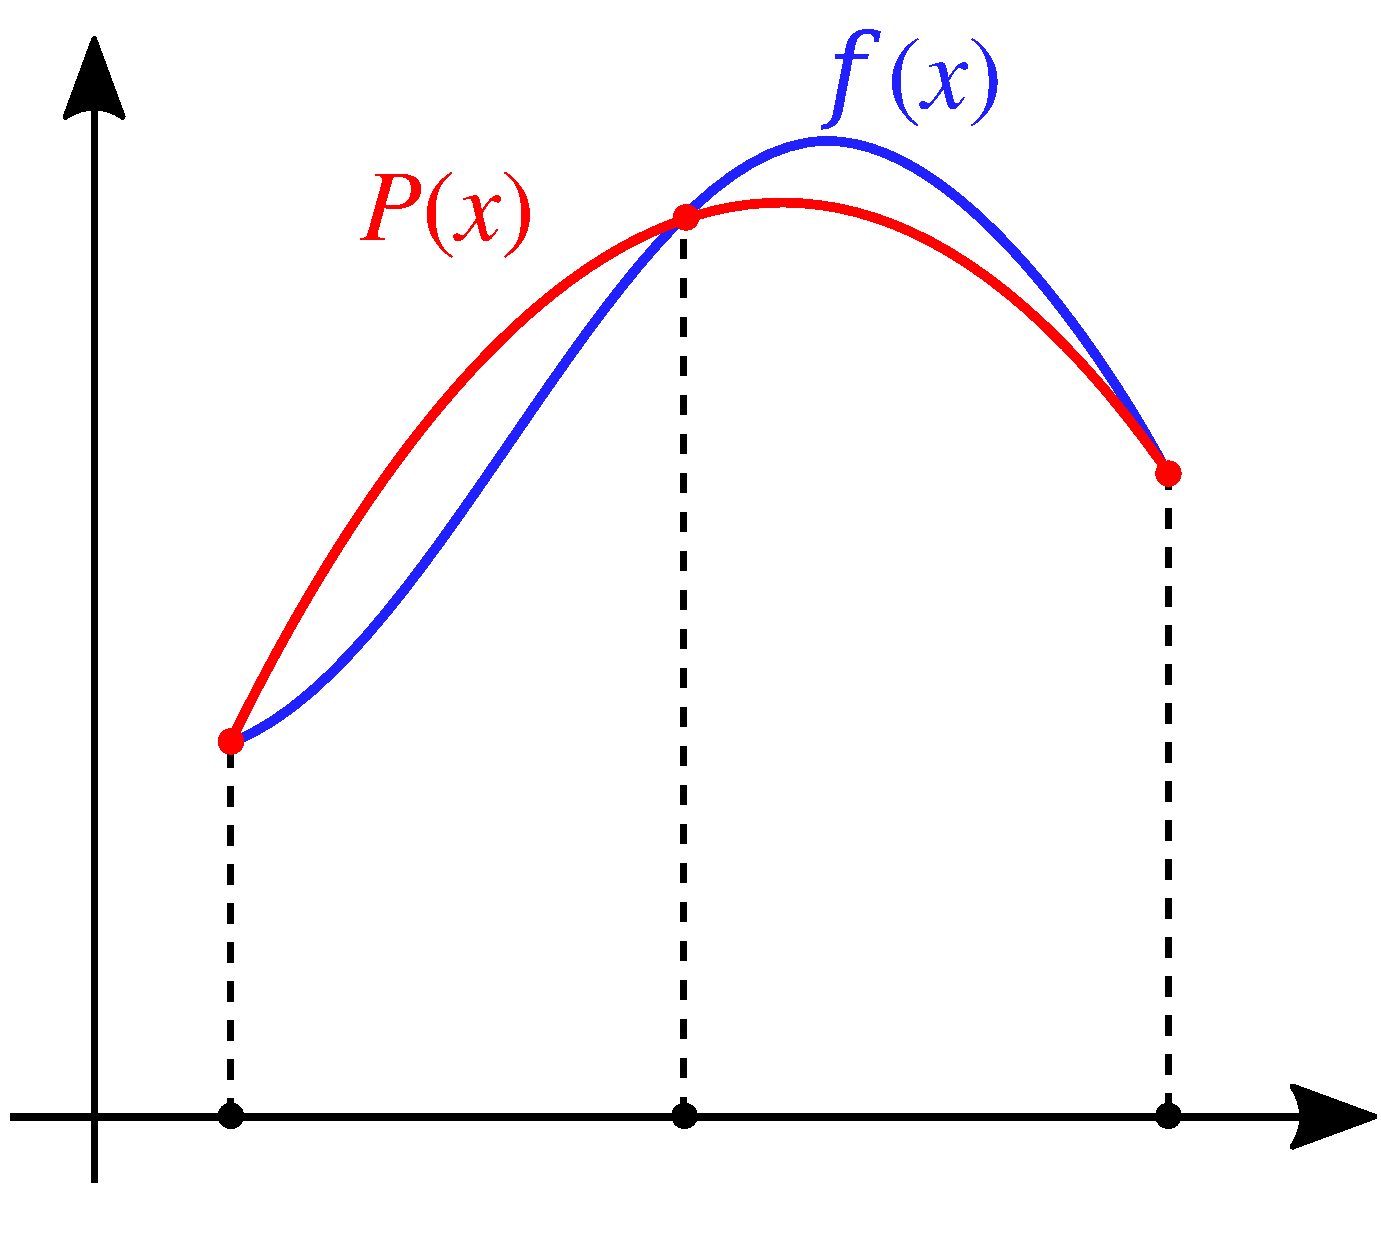
\includegraphics[width = \linewidth]{Simpson's Rule.pdf}
%   \end{center}
%   \caption{}
%   \label{fig:simpsonsrule}
% \end{wrapfigure}
Simpson's Rule is a method in numerical integration (approximating definite integrals).\\
It approximates the area of $f(x)$ in the interval $[a,b]$ by area of parabola passing through $a, \mfrac{a+b}{2}, b$. as shown in \ref{fig:simpsonsrule}.%\footnote{\href{https://bit.ly/simpsonsrule}{Image source}}.%\ref{fig:simpsonsrule}
\begin{figure}[H]
\centering
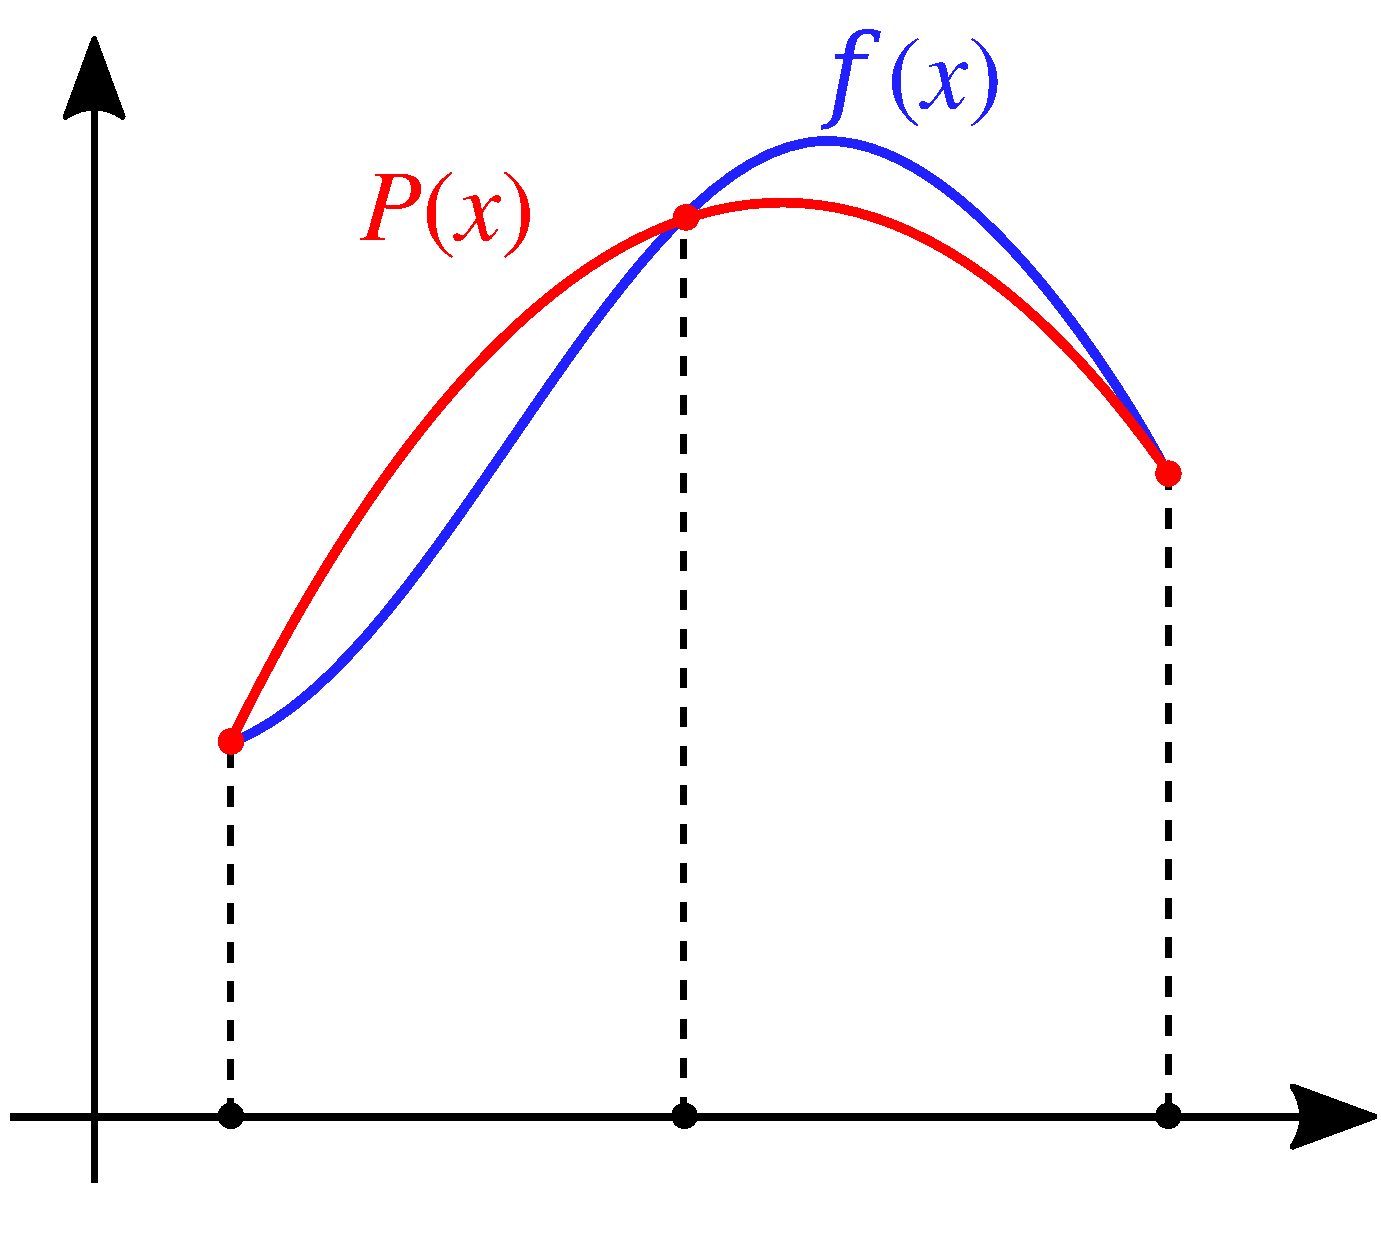
\includegraphics[width = 0.2\linewidth]{Simpson's Rule.pdf}
\caption{Approximating $f(x)$ by a parabola $P(x)$. \href{https://bit.ly/simpsons-rule}{(Image Source)}}
\label{fig:simpsonsrule}
\end{figure}
\begin{equation}{\label{eq:cs}}
{ \int _{a}^{b}f(x)\,dx\approx {\frac {b-a}{6}}\left[f(a)+4f\left({\frac {a+b}{2}}\right)+f(b)\right]}
\end{equation}
If \ref{eq:cs} is applied to $n$ equally spaced subdivisions in $[a, b]$, we get the \emph{composite Simpson's rule} \ref{eq:csr}.
\begin{equation}{\label{eq:csr}}
	 \int _{a}^{b}f(x)\,dx\approx {\frac {\Delta x}{3}}\left(f(x_{0})+4f(x_{1})+2f(x_{2})+4f(x_{3})+2f(x_{4})+\cdots +4f(x_{n-1})+f(x_{n})\right)
\end{equation}
where each of the $n+1$ ordinates is given by $x_i = a+i\Delta x$ for $i = 0,1,\ldots,n$ and $\Delta x = \mfrac{b-a}{n}$
\begin{note}
	Simpson's rule can only be applied when an odd number of ordinates is chosen.
\end{note}
\textbf{Problem Statement:}\\
\begin{equation}{\label{eq:pi_integral}}
{ \pi={22 \over 7} - \int _{0}^{1}{x^{4}(1-x)^{4} \over 1+x^{2}}\,dx } 
\end{equation}
% $\pi$ can be approximated using \ref{eq:pi_integral}\\
% \begin{equation*}{\label{eq:simp}}
% 	x = \int_{0.5}^{1}\frac{\sin\theta}{\theta}\d\theta
% \end{equation*}
Calculate $\pi_n$ (approximate \ref{eq:pi_integral} using $n$ ordinates) for all test cases (accurate till 15 decimal places).% See Starter code (below) for more details.
\begin{testcases}
	{$t$ \hfill(number of test cases, an integer)\\$n_1\ n_2\ \ldots\ n_t$ \hfill($t$ space seperated integers for each testcase)}
	{$\pi_{n_i}$ \hfill(each test case on a newline, accurate till 15 decimal places)}
	{$0 < n_i < 500$ and $n_i$ is odd}
	{10\\3 5 7 11 15 31 57 99 163 441}
	{3.140773809523810\\3.141684884891457\\3.141601987350571\\3.141593090129691\\3.141592711563659\\3.141592654188570\\3.141592653603947\\3.141592653590286\\3.141592653589817\\3.141592653589793}
	{https://github.com/paramrathour/CS-101/tree/main/Starter Codes/Simpson's Rule.cpp}
\end{testcases}
}
